% Completa los datos convenientemente en las zonas marcadas con TODO

\documentclass{beamer}
%PARA VISUALIZAR PRESENTACIONN CON NOTAS USAR VISUALIZADOR "pdfpc":
%Para ver las notas, el cronometro y siguente diapo:
% pdfpc --notes=right slides.pdf
% "tecla p": para pausar el cronometro
\mode<presentation> {
  \usetheme{CambridgeUS}
  \usecolortheme{crane} % color naranja
}

\definecolor{mypink}{RGB}{250,181,235}
\definecolor{mygreen}{RGB}{186, 242, 187}
\definecolor{mymint}{RGB}{186, 242, 216}
\definecolor{myred}{RGB}{236, 64, 103}

\setbeamercolor*{structure}{bg=mypink!20,fg=mypink}

\setbeamercolor*{palette primary}{use=structure,fg=white,bg=structure.fg}
\setbeamercolor*{palette secondary}{use=structure,fg=white,bg=structure.fg!75} %fondo de abajo en medio
\setbeamercolor*{palette tertiary}{use=structure,fg=white,bg=black} %fondo de la izquierda
%\setbeamercolor*{palette quaternary}{fg=white,bg=black}

%\setbeamercolor{section in toc}{fg=black,bg=white}
\setbeamercolor{alerted text}{use=structure,fg=structure.fg!50!black!80!black}

%\setbeamercolor{titlelike}{parent=palette primary,fg=structure.fg!50!black}
\setbeamercolor{frametitle}{bg=mypink!85,fg=white} %Barra de titulo (contenidos, etc)

\setbeamercolor*{titlelike}{use=structure,fg=black,bg=mypink!70}
\setbeamercolor{item projected}{fg=black,bg=mypink}

%\definecolor{mypink}{RGB}{250,181,235}
%\setbeamercolor*{structure}{bg=mypink!20,fg=mypink}

%\setbeamercolor*{palette primary}{use=structure,fg=white,bg=structure.fg}
%\setbeamercolor*{palette secondary}{use=structure,fg=white,bg=structure.fg!75}


%\setbeamercolor{titlelike}{parent=structure,bg=mypink,fg=structure.fg!50!black}
%\setbeamercolor{frametitle}{bg=mypink!85,fg=white}
%\setbeamercolor{section in toc}{fg=black,bg=white}

%\setbeamercolor{titlelike}{parent=structure,bg=mypink} % Cambia el color de la caja del título de la página inicial

\setbeamertemplate{navigation symbols}{} % ocultar iconos de navegación
\setbeamerfont{subsection in toc}{size=\small} % reducir tamaño en TOC
\setbeamerfont{date}{size=\tiny}
\usepackage[spanish]{babel}
\usepackage[utf8]{inputenc}
\usepackage{graphicx}
\usepackage{booktabs}
\usepackage{hyperref}
\usepackage{multicol}
\usepackage{pgfpages}
\usepackage{listings}
\usepackage{multimedia}
\usepackage[export]{adjustbox}
\usepackage{outlines} % Para poner bullets tabulados (\1 \2 \3 ...) y no items

\usepackage{array,tabularx} % para tabular leyenda de ecuaciones
\newenvironment{conditions*} % entorno de "leyenda de ecuación"
  {\par\vspace{\abovedisplayskip}\noindent
   \tabularx{\columnwidth}{>{$}l<{$} @{\ : } >{\raggedright\arraybackslash}X}}
  {\endtabularx\par\vspace{\belowdisplayskip}}
  
% USO DE NOTAS
\setbeameroption{show notes} % Para mostrar u ocultar (hide/show)
%\setbeameroption{show only notes} % Mostrar solo las notas
\setbeameroption{show notes on second screen=right} % Mostrar notas en otra pantalla
\setbeamertemplate{note page}{ % asi solo muestro el texto de las notas
  \insertnote%
}

%========= TODO: datos internos del documento
\hypersetup{
	pdftitle={Defensa de trabajo de fin de grado de Isabel Cebollada Gracia},
	pdfauthor={Isabel Cebollada Gracia},
	pdfsubject={Sistema de monitorización para el control y estudio del bienestar de animales de laboratorio mediante una infraestructura de bajo coste},
	pdfkeywords={raspberry, inteligencia artificial, machine learning, deep learning, visión artificial},
	pdfproducer={pdfLaTeX},
  colorlinks=true,
  linkcolor=blue
}
%=========

%========= TODO: diapositiva de portada
\title[Sistema de monitorización]{Sistema de monitorización para el control y estudio del bienestar de animales de laboratorio mediante una infraestructura de bajo coste} % El título reducido aparece en la parte inferior de todas las diapositivas
                                         % El título completo aparece solo en la diapositiva de portada
\author[Isabel Cebollada Gracia]{Isabel Cebollada Gracia}
\institute[URJC]
{
\textit{\href{mailto:i.cebollada.2018@alumnos.urjc.es}{\color{blue}{\underline{i.cebollada.2018@alumnos.urjc.es}}}}\\
\vspace{0.5cm}

\includegraphics[width=3cm]{figs/logo-urjc}\\
\vspace{1cm}
Trabajo fin de grado
}
\date{27 de Julio de 2022}
%=========

%========= COMIENZO DEL DOCUMENTO
\begin{document}

%========= Portada inicial con notas
\begin{frame}[plain] % plain: quita header y footer
\large{\titlepage}
\note[item]{En esta presentación voy a hablar sobre...}
\note[item]{En primer lugar...}
\end{frame}

%========= Licencia
\begingroup
\hypersetup{linkcolor=white}
\begin{frame}
% Este diseño se corresponde con la licencia CC-BY-NC-SA.
% Por supuesto, puedes poner la licencia que mejor se adapte al propósito de tu trabajo.
% Recuerda que, si no se especifica ninguna licencia, esta -como cualquier creación artística- pasaría a estar licenciada con todos los derechos reservados (copyright).

\cleardoublepage

\begin{figure}
 \ \ \ \ 
\includegraphics[width=0.25\linewidth]{figs/by-nc-sa.png}
 \label{fig:cc} 
 \end{figure}

\

\

\

\noindent
Este trabajo se distribuye bajo los términos de la licencia internacional \href{http://creativecommons.org/licenses/by-nc-sa/4.0/}{CC BY-NC-SA International License} (Creative Commons AttributionNonCommercial-ShareAlike 4.0). Usted es libre de \textit{(a) compartir}: copiar y redistribuir el material en cualquier medio o formato; y \textit{(b) adaptar}: remezclar, transformar y crear a partir del material. El licenciador no puede revocar estas libertades mientras cumpla con los términos de la licencia:

\begin{itemize}
\item \textit{Atribución}. Usted debe dar crédito de manera adecuada, brindar un enlace a la licencia, e indicar si se han realizado cambios. Puede hacerlo en cualquier forma razonable, pero no de forma tal que sugiera que usted o su uso tienen el apoyo de la licenciante.
\item \textit{No comercial}. Usted no puede hacer uso del material con propósitos comerciales.
\item \textit{Compartir igual}. Si remezcla, transforma o crea a partir del material, debe distribuir su contribución bajo la la misma licencia del original.
\end{itemize}

\begin{flushright}
		\vspace{7.0 cm}
		\emph{Documento de} \textbf{Isabel Cebollada}. % TODO: pon aquí tu nombre cuando hagas el documento
\end{flushright}


\end{frame}
\endgroup

%========= Índice o tabla de contenidos (TOC)
\begin{frame}
\frametitle{Contenidos}
%\begin{multicols}{2} % si tengo muchas secciones, lo parte en dos columnas
  \tableofcontents[hideallsubsections] % no muestra subsecciones
%\end{multicols}
\note[item]{La presentaci\'on esta dividida en cuatro partes.}
\end{frame}

\begingroup
\hypersetup{linkcolor=white}
%========= Diapositiva "vacía" de comienzo de sección:
\section*{}
\begin{frame}{}
  \centering \Huge
  \emph{Introducción}
\note[item]{Comencemos con la introducción a la robótica.}
\end{frame}

\section{Introducción}
\subsection{Contexto del trabajo}
%========= Diapositiva con imágenes:
\begin{frame}
\frametitle{Introducción a la robótica}
¿Qué es la robótica?
\begin{itemize}
\item Campo de investigación muy importante que continua en desarrollo.
\item Objetivo: Realizar trabajos \textcolor{myred}{aburridos} o \textcolor{myred}{pesados} para el humano.
\end{itemize}
\note[item]{La robótica es un campo de investigación muy importante en la actualidad que continua en desarrollo, cuyo objetivo es realizar trabajos que resultan pesados, aburridos o sucios para el ser humano.}
\end{frame}
\begin{frame}
\frametitle{Definición de robot}
¿Qué es un robot?
\begin{figure}
\centering
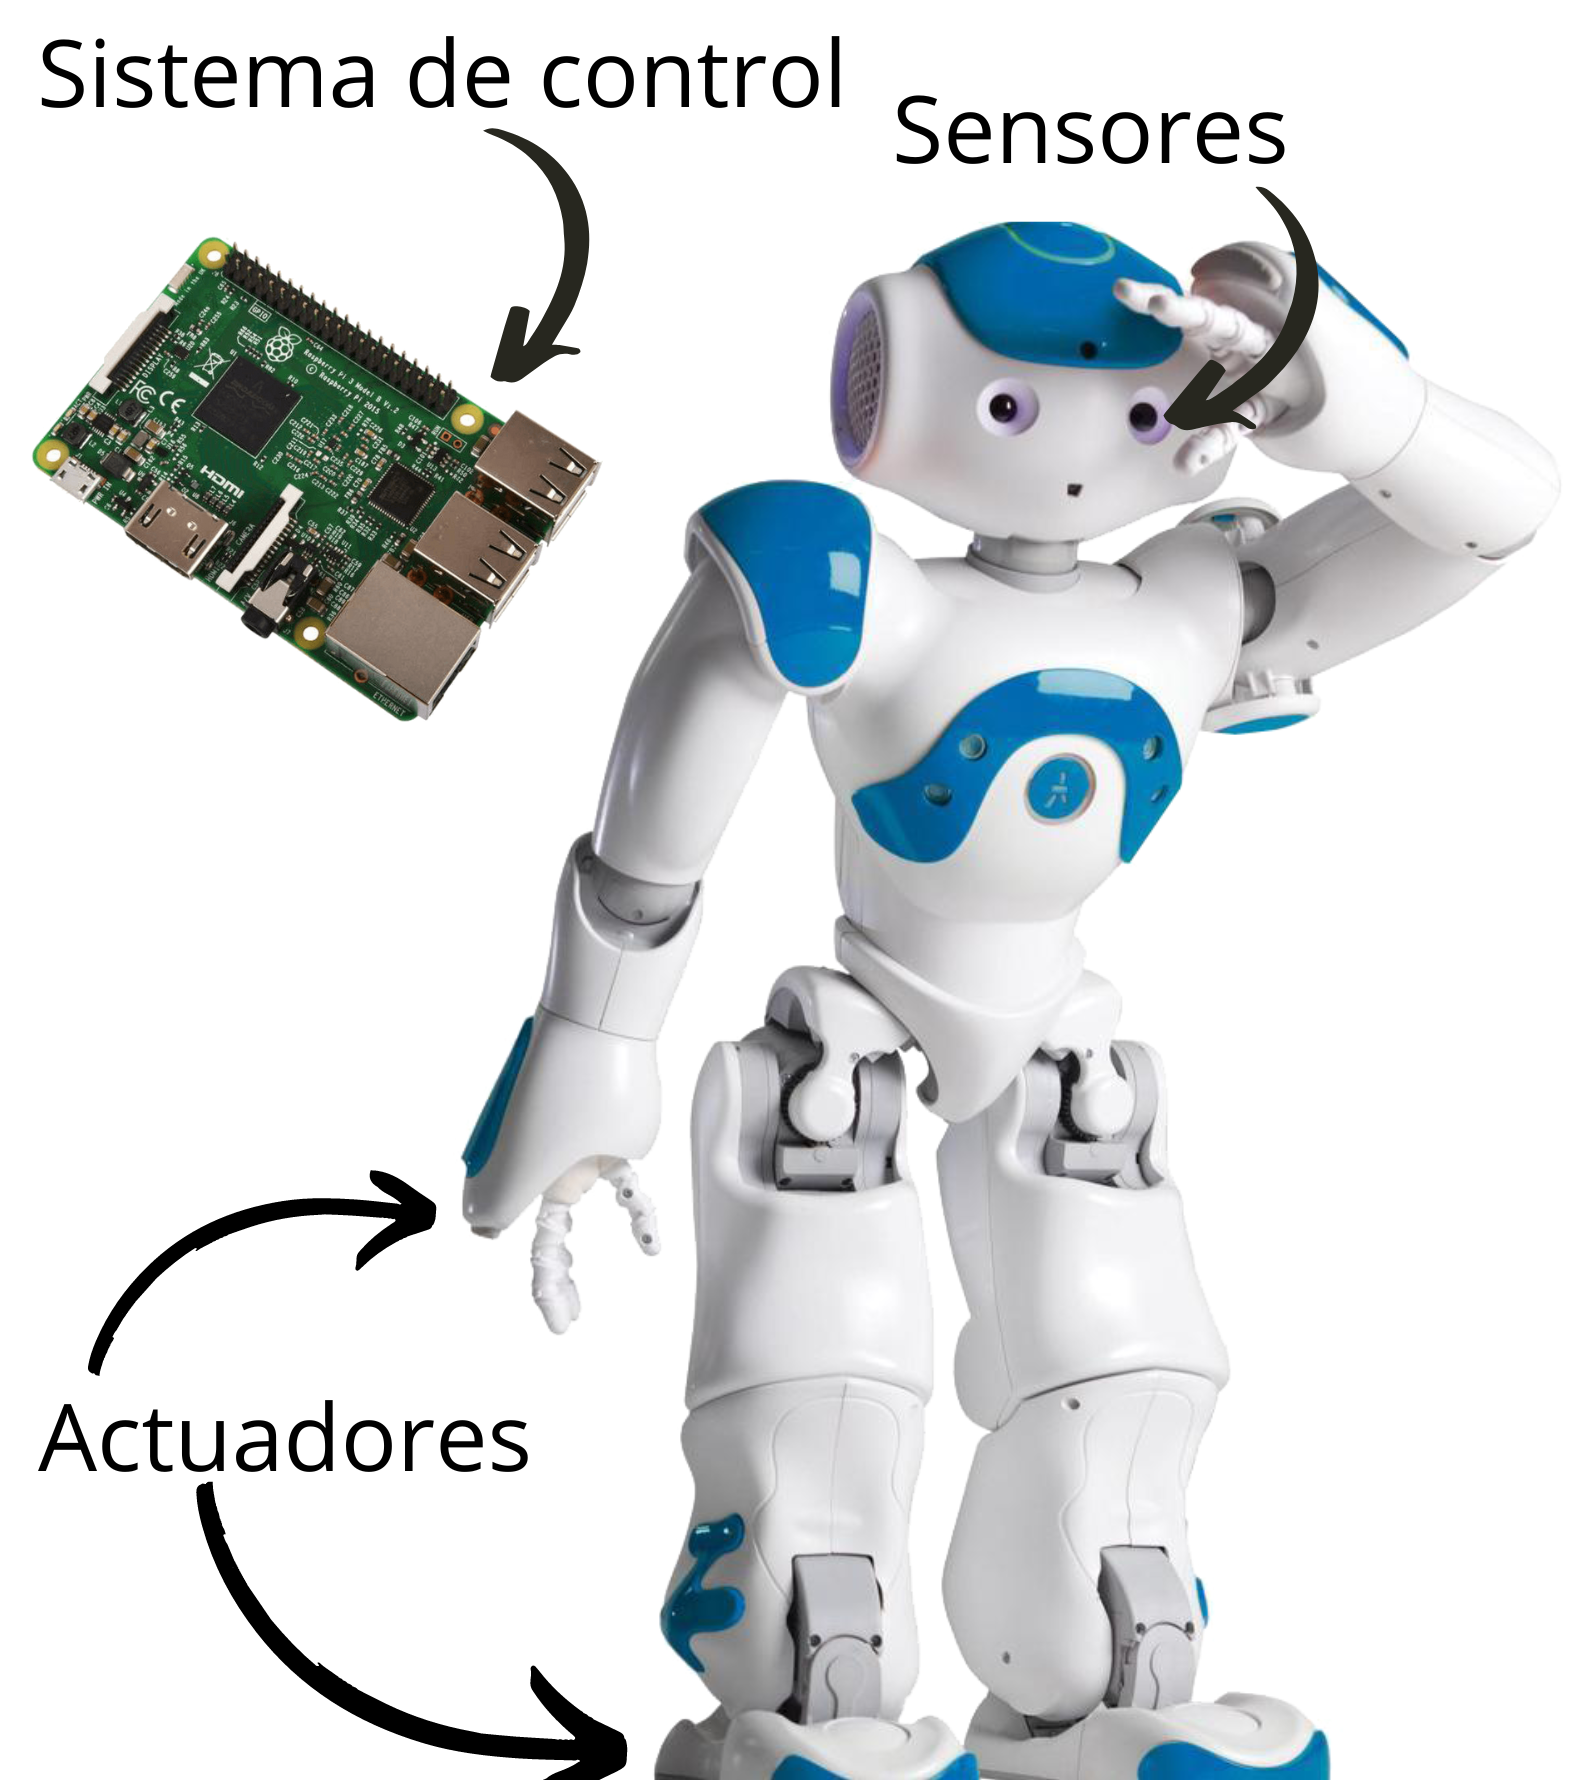
\includegraphics[width=6.32cm]{figs/robot}
\end{figure}
\note[item]{A lo largo de los años el concepto de robótica ha ido variando, así como la definición de robot. Actualmente, se entiende por robot a cualquier dispositivo dotado por sensores, actuadores y un sistema de control.}
\end{frame}

\begin{frame}
\frametitle{Algunos tipos de sensores}
\begin{figure}
\centering
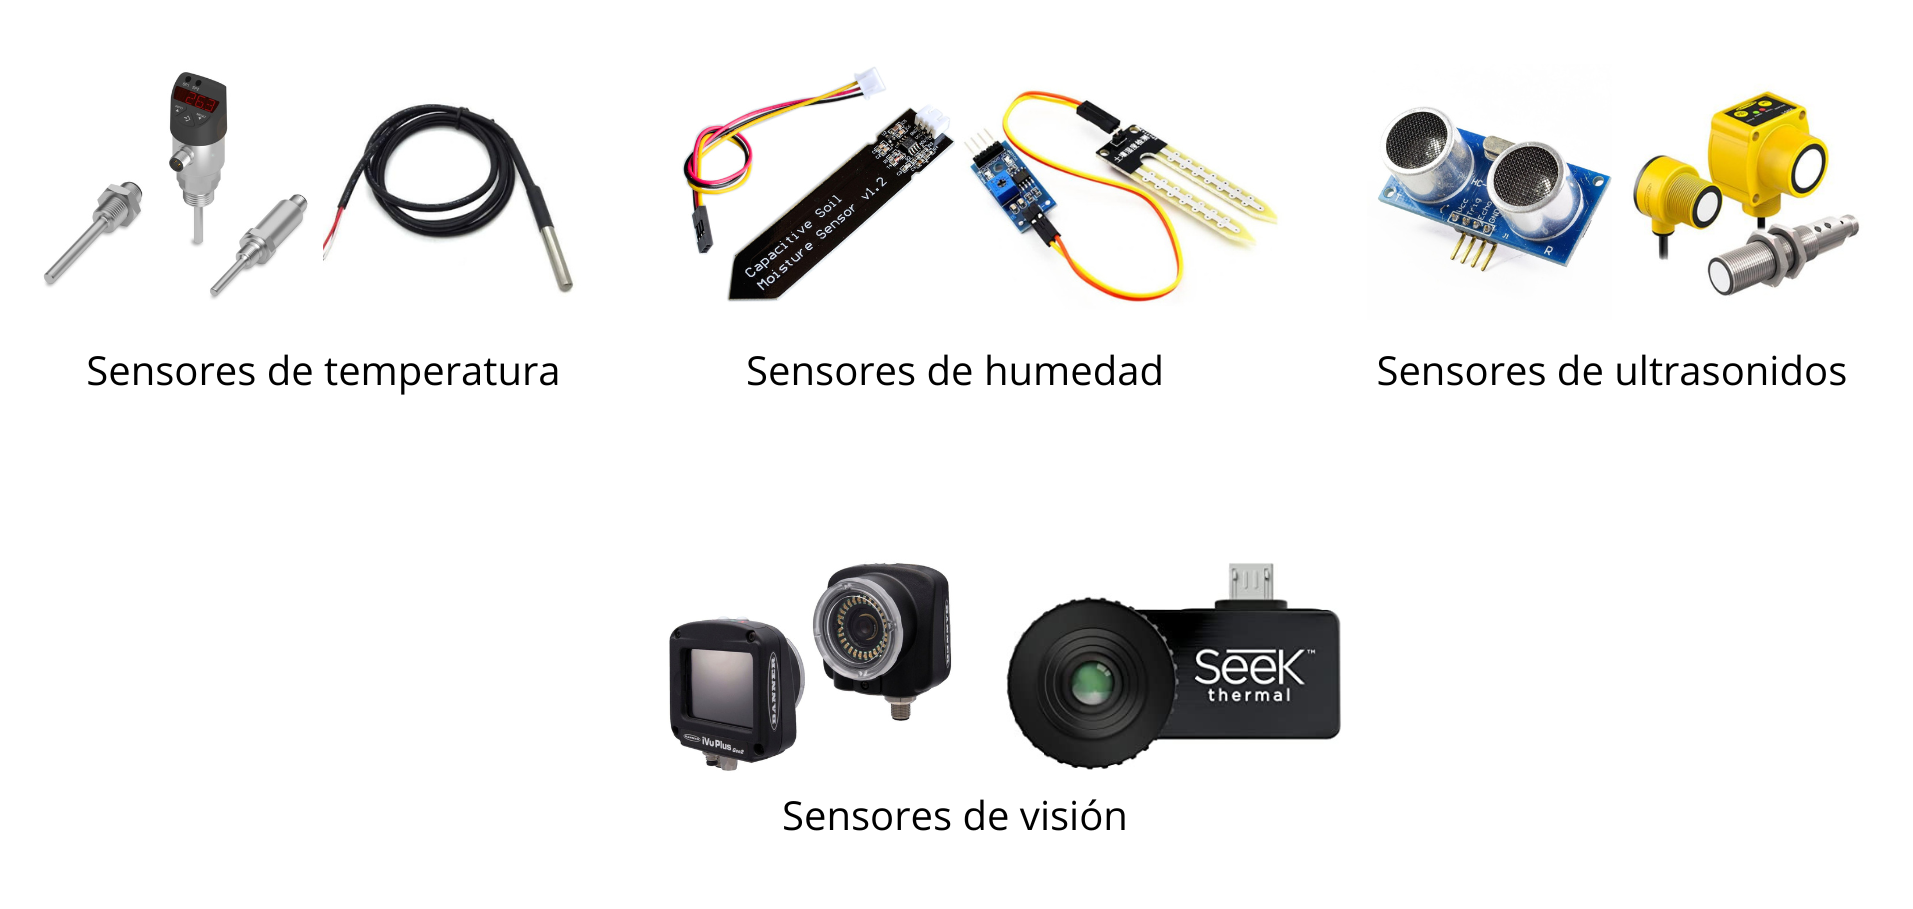
\includegraphics[width=12cm]{figs/sensores}
\end{figure}
\note[item]{Existen distintos tipos de sensores que dotan de distintas cualidades. Entre ellos, uno de los más importantes es el sensor de visión, que requiere un proceso arduo para extraer información útil en tiempo real. Para el procesamiento de la información obtenida del sensor de visión, es necesario aplicar un algoritmo de IA.}
\end{frame}

\begin{frame}
\frametitle{Inteligencia Artificial}
\begin{figure}
\centering
\includegraphics[width=7cm]{figs/ia-5}
\end{figure}
\note[item]{La inteligencia artificial consiste en replicar los mecanismos del cerebro mediante algoritmos. Uno de los algoritmos más usados es el ML, preprogramados por un humano y que tratan de descubrir patrones que les hacen aprender. Los algoritmos más usados en visión artificial pertenecen a un subcampo del ML denominado DL, donde el autómata aprende por si mismo sin intervención humana, simulando el cerebro con unidades equivalentes a las neuronas.}
\end{frame}

\begin{frame}
\frametitle{Sistemas multisensoriales}
\begin{figure}
\centering
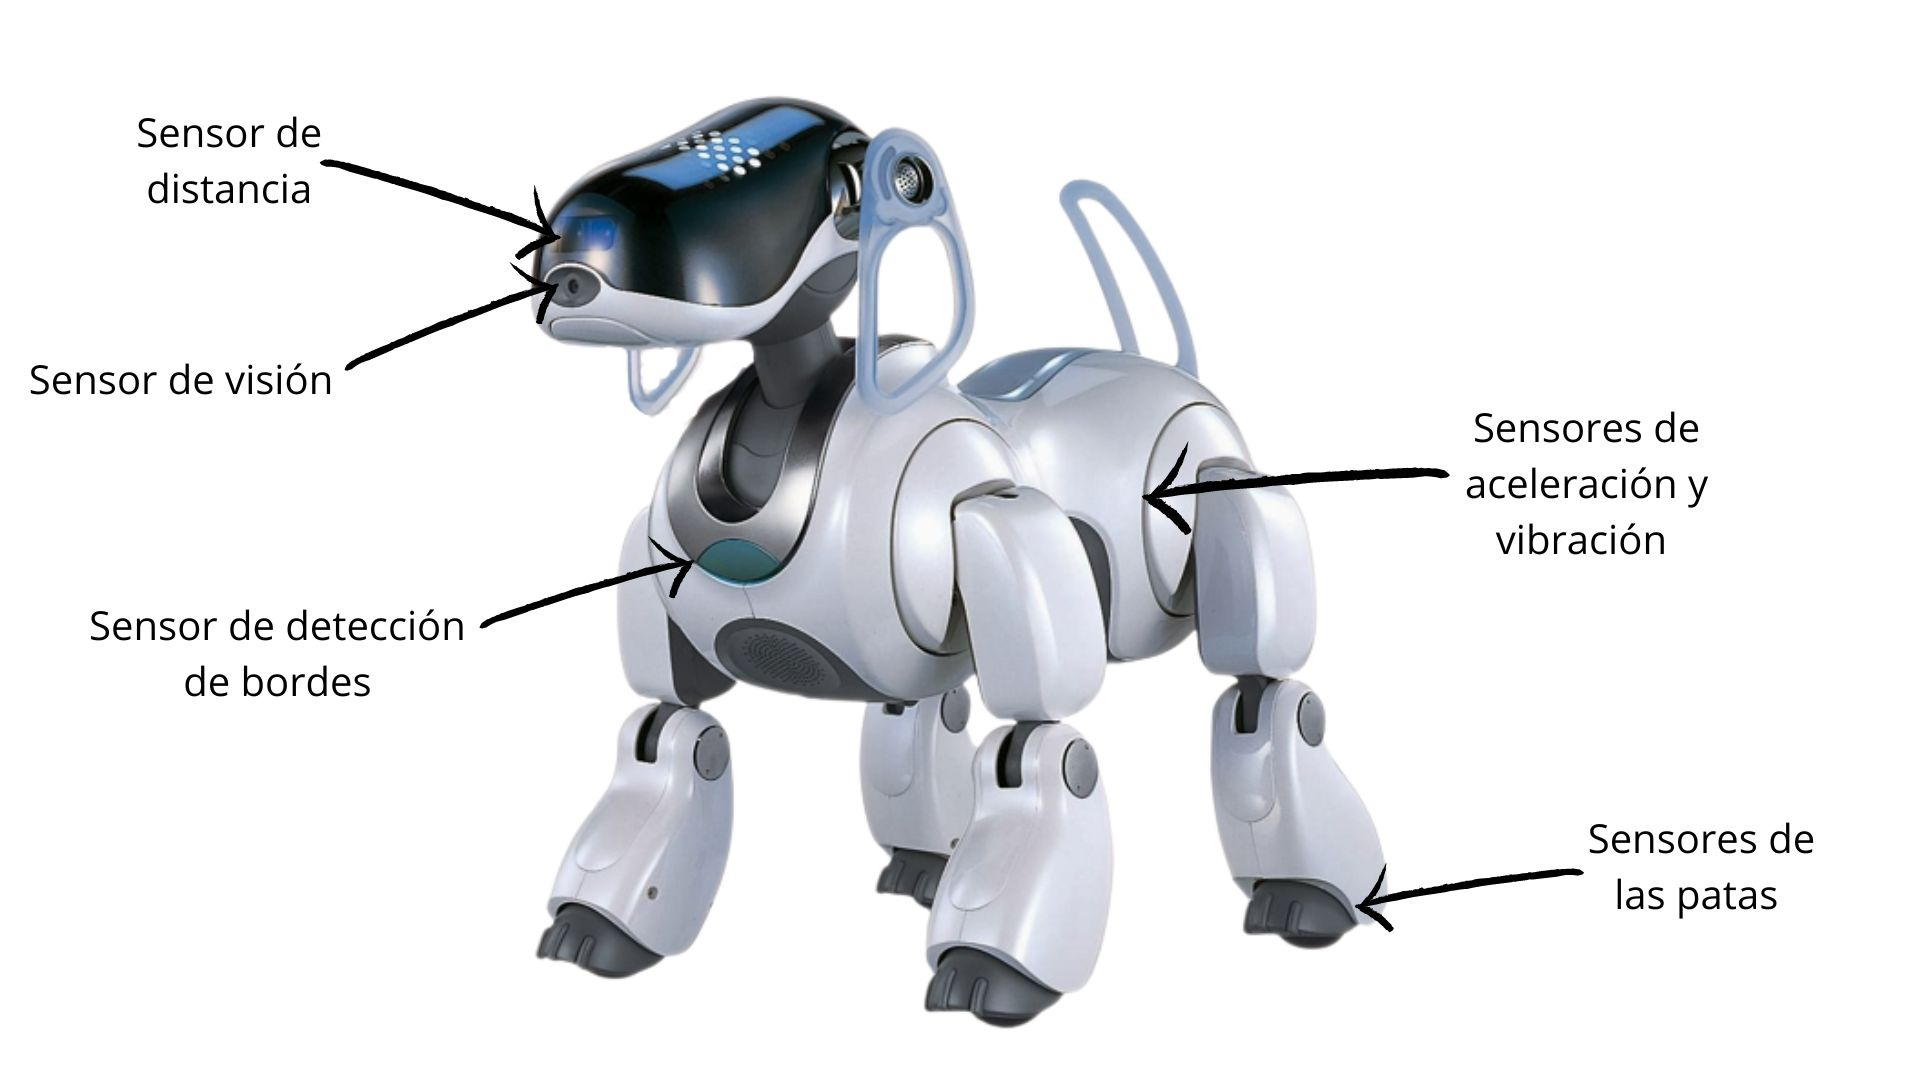
\includegraphics[width=12cm]{figs/multisensorial}
\end{figure}
\note[item]{Además de utilizar sensores de visión, si a un robot se le incorporan diferentes tipos de sensores, este obtendrá mucha más información, por lo que podrá ser más preciso y simular a un humano mejor. Este trabajo se enmarca en el contexto de los sistemas multisensoriales, concretamente en los sistemas multisensoriales destinados al bienestar animal y al análisis de comportamiento.}
\end{frame}

%------------------------------------------------------------------------------OBJETIVOS------------------------------------------------------------------------------
%
%%========= Diapositiva con ítems resaltados con colores:
%\begin{frame}
%\frametitle{Introducción a la Robótica}
%\begin{itemize}
%\item La \textcolor{red}{tecnología} está cada vez más presente en la vida cotidiana.
%\item Los robots de servicio aparecen en el \textcolor{blue}{mercado}.
%\item La \textcolor{red}{domótica} presenta cada vez más aplicaciones domésticas.
%\end{itemize}
%\end{frame}
%
%\subsection{Contexto específico}
%%========= Diapositiva con bloques:
%\begin{frame}
%\frametitle{Precedentes de la robótica}
%\begin{block}{Primera revolución industrial de 1800}
%Productos fabricados por \textcolor{blue}{máquinas}. La \textcolor{red}{máquina de vapor} fue clave.
%\end{block}
%\end{frame}
%
%%========= Diapositiva con bullets en diferentes niveles (outline):
%\section{Principios de transducción}
%\subsection{Principio de transducción piezoresistivo}
%\begin{frame}
%\frametitle{Conceptos}
%\begin{outline}
%\1 Piezoresistividad: relación entre resistencia eléctrica y deformación.
%\2 Material piezoresistivo: (1) material en reposo (átomos en equilibrio).
%\3 (2) Si sufre deformación, movimiento átomos, modifican su resistividad.
%\2 Resistencia vs. resistividad de un material.
%\3 Resistencia: depende del volumen del material a tratar.
%\3 Resistividad: caract. intrínseca relacionada con colocación de átomos.
%\end{outline}
%\end{frame}
%

\section*{}
\begin{frame}{}
  \centering \Huge
  \emph{Objetivos}
\note[item]{Pasemos ahora a comentar los objetivos que nos hemos marcado con este trabajo.}
\end{frame}

\setbeamercolor{block title}{bg=mypink!40,fg=black}


\section{Objetivos}
\begin{frame}
\begin{block}{Objetivos}
\begin{itemize}
\item Recoger la lectura de los sensores en paralelo en un mismo fichero.
\item Crear un servidor web para los sensores de las cámaras.
\item Detectar los ratones mediante algoritmos de Deep Learning.
\end{itemize}
\end{block}

\begin{block}{Requisitos}
\begin{itemize}
\item El sistema debe ser capaz de ejecutar en tiempo real sobre Raspberry.
\item El lenguaje de programación debe ser Python.
\item La interfaz de usuario se creará en Node-Red.
\end{itemize}
\end{block}
\end{frame}

%\section{Objetivos}
%%\subsection{Objetivos}
%\begin{frame}
%\begin{enumerate}
%\item Recoger la lectura de los sensores en paralelo en un mismo fichero.
%\item Crear un servidor web para los sensores de las cámaras.
%\item Detectar los ratones mediante algoritmos de Deep Learning.
%\end{enumerate}
%\note[item]{Los objetivos marcados para realizar el proyecto son los siguientes.}
%\end{frame}
%
%\section{Objetivos}
%\subsection{Requisitos}
%\begin{frame}
%\begin{figure}
%\centering
%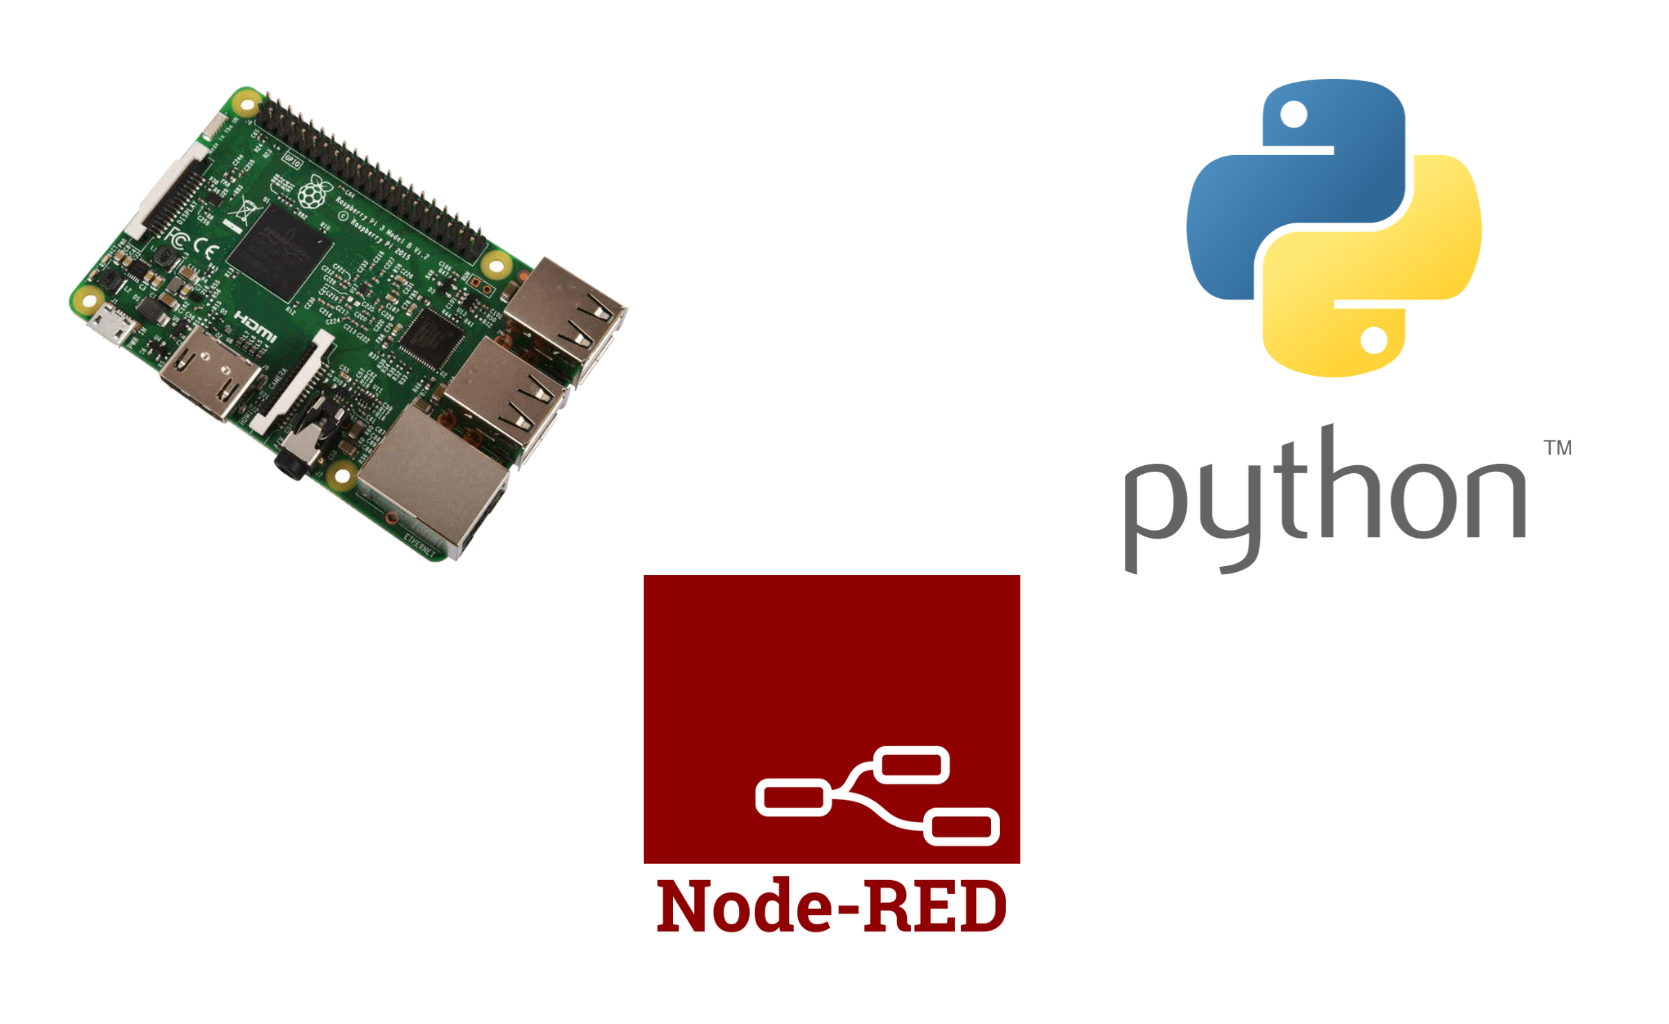
\includegraphics[width=12cm]{figs/requisitos}
%\end{figure}
%\note[item]{Los requisitos para cumplir dichos objetivos son los siguientes: Que el sistema sea capaz de ejecutar en tiempo real sobre Raspberry Pi 4B. Que el lenguaje de programación sea Python, ya que es sencillo y ofrece múltiples librerías útiles para este trabajo, además que está soportado completamente por el SO de Raspberry. Finalmente, la IU se creará con Node-Red, una herramienta muy visual creada para dispositivos embebidos.}
%\end{frame}


%---------------------------------------------------------------------------DISEÑO-----------------------------------------------------------------------------
\section*{}
\begin{frame}{}
  \centering \Huge
  \emph{Diseño}
\note[item]{Una vez descritos los objetivos, veamos la infraestructura y plataformas utilizadas.}
\end{frame}

\section{Plataforma de desarrollo}
\subsection{Infraestructura hardware}
\begin{frame}
\frametitle{Infraestructura hardware}
\begin{figure}
\centering
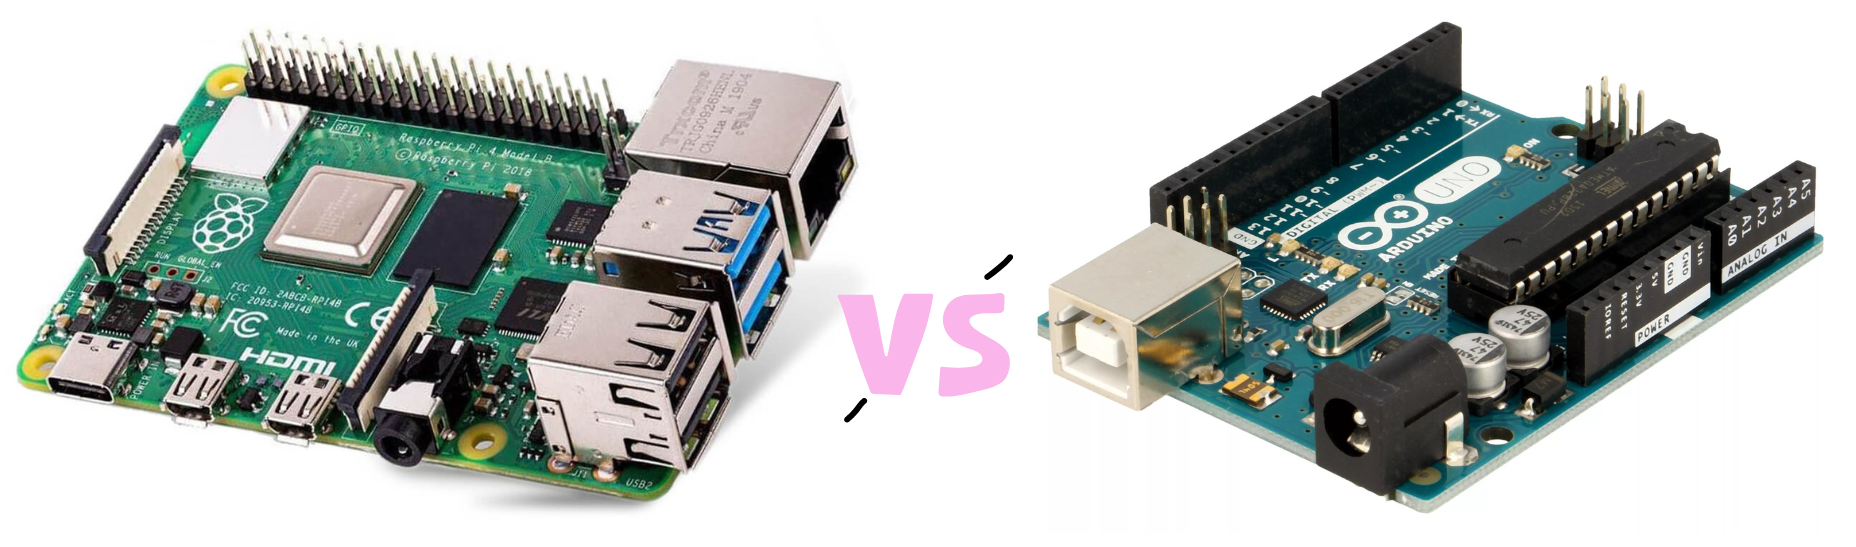
\includegraphics[width=12cm]{figs/VS}
\end{figure}
\begin{multicols}{2}

\begin{itemize}
\centering
\item[] Pines GPIO
\item[] Conexión de cámaras
\item[] Cuatro puertos USB
\item[] Dos puertos micro-USB
\item[] Microordenador
\item[] Sistema operativo completo
\item[] Pines GPIO
\item[] No conexión de cámaras
\item[] No tiene puertos USB
\item[] No tiene puertos micro-USB
\item[] Microprocesador
\item[] IDE
\end{itemize}

\end{multicols}
\note[item]{Existen distintos sistemas embebidos que se podrían haber utilizado para este trabajo. Los dos más conocidos son Raspberry y Arduino. Hay varias características favorables a Raspberry que han hecho que se seleccione esta placa frente a Arduino.}
\end{frame}

\subsection{Infraestructura hardware}
\begin{frame}
\begin{figure}
\centering
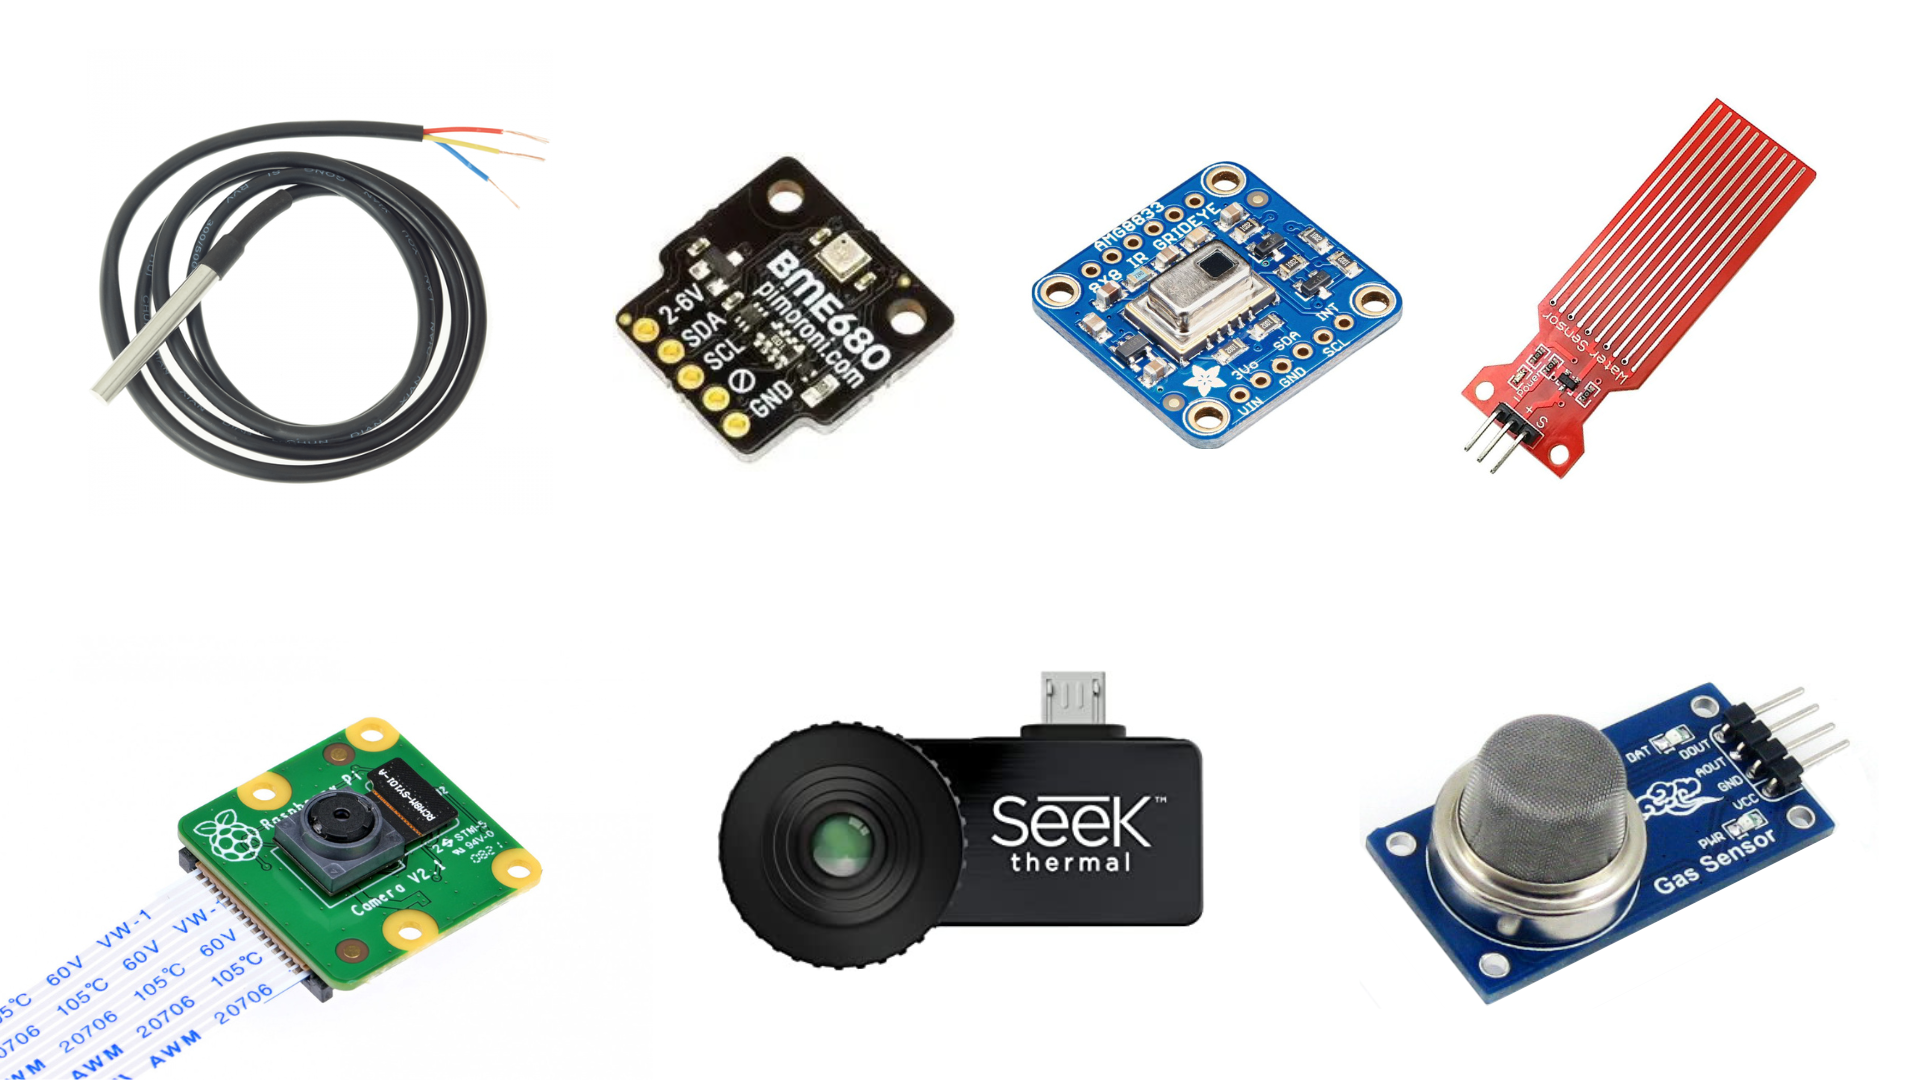
\includegraphics[width=12cm]{figs/sensoresusados}
\end{figure}
\note[item]{A través de los múltiples pines, se han conectado los sensores utilizados para el funcionamiento del sistema. El sensor DS18B20, arriba a la izquierda, permite medir la temperatura. Es resistente al agua, así que permite la medición en superficies húmedas o mojadas. Continuando a la derecha se encuentra el sensor BME680 permite medir cuatro parámetros: temperatura, humedad, presión y resistencia del aire. El sensor AMG8833 es un sensor térmico, que obtiene un mapa de 8x8 valores numéricos referentes a las temperaturas. El siguiente sensor, arriba a la derecha es un sensor que permite medir el nivel de agua. Empezando por la izquierda en la fila de abajo se encuentra la PiCam, una de las cámaras oficiales de raspberry que permite la visión del entorno. A su derecha está la Seek Thermal cam, que es una cámara térmica, originalmente creada para el uso en teléfonos móviles pero que permite su conexión a raspberry por el puerto USB con un adaptador. Finalmente, abajo a la derecha está en MQ-135, un sensor que permite detectar la concentración de ciertos gases en el aire, como el amoníaco.}
\end{frame}

\subsection{Infraestructura software}
\begin{frame}
\frametitle{Infraestructura software}
\begin{figure}
\centering
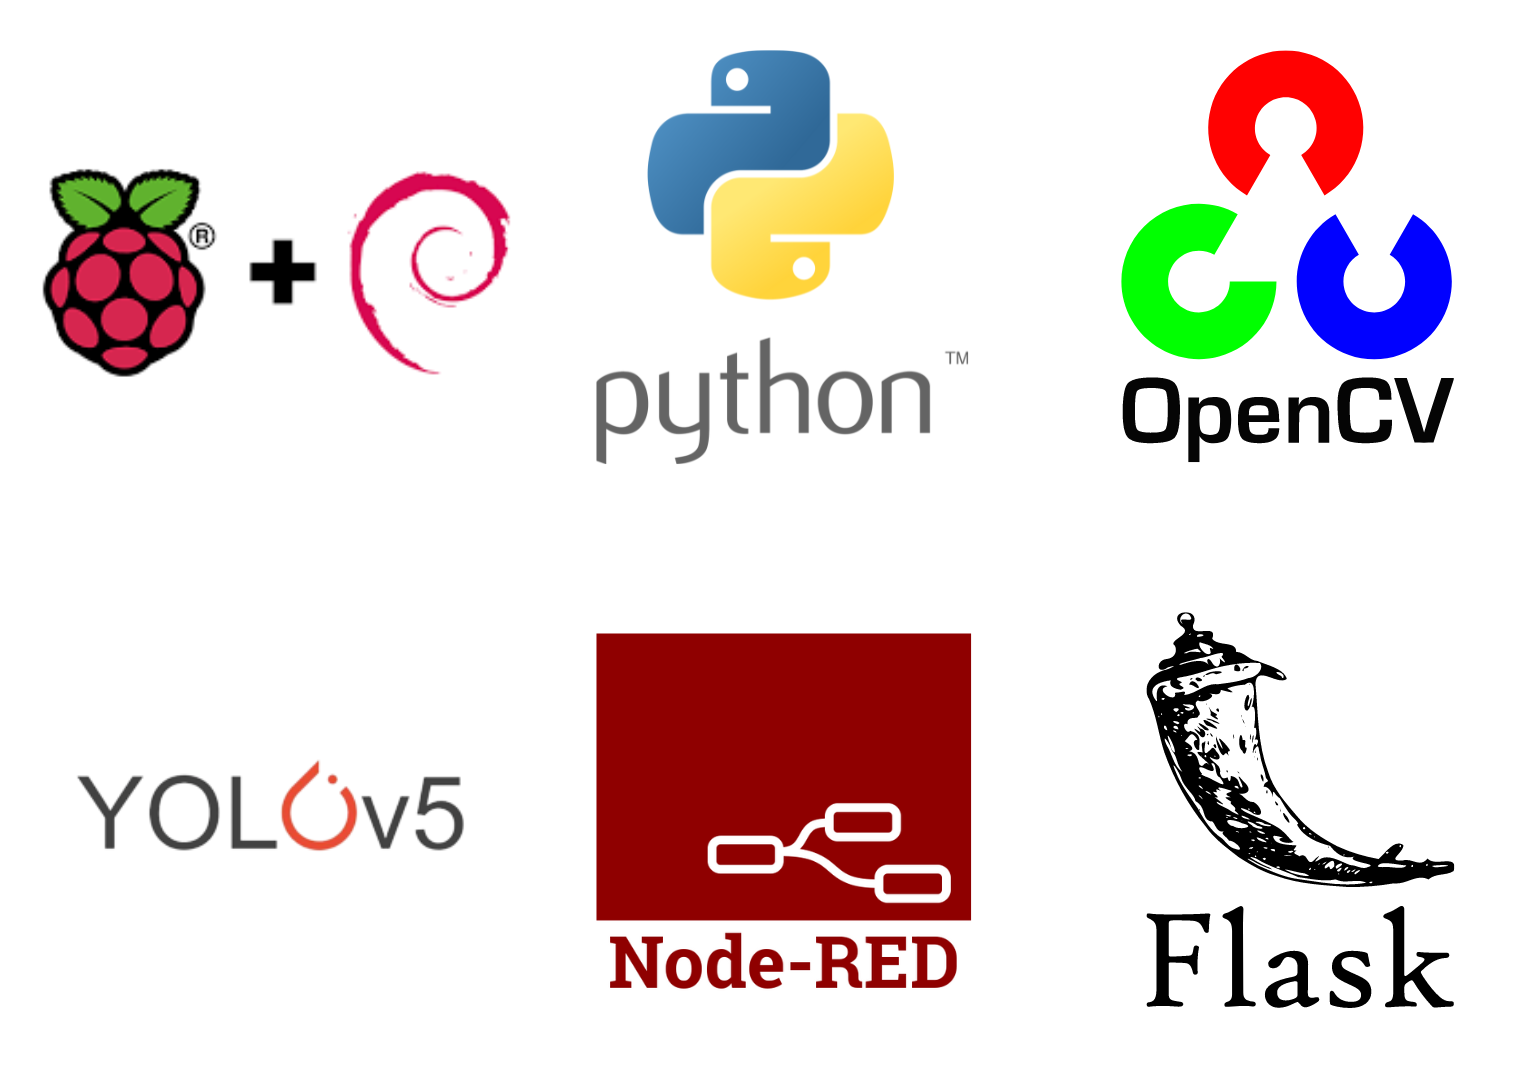
\includegraphics[width=10cm]{figs/apps}
\end{figure}
\note[item]{Como ya he presentado se utiliza para el desarrollo de este sistema la placa Raspberry. El sistema operativo que se ha usado en esta placa es Raspbian, basado en Debian, bajo la versión de 64 bits. El lenguaje seleccionado ha sido Python, debido a que está soportado de forma nativa en el SO, que es uno de los lenguajes más usados actualmente y que posee numerosas librerías útiles para el proyecto desarrollado. Una de ellas es OpenCV, que permite la manipulación de los vídeos. Se ha utilizado para realizar algunas modificaciones con la cámara, como añadir un timestamp así como para la detección de ratones. Para dicha detección, previamente ha sido necesario utilizar yolo para crear un modelo de detección de ratones. Por otro lado, para la creación de la IU se ha utilizado Node-Red, como previamente se estableció en los requisitos, y Flask para crear los servidores web.}
\end{frame}

%-----------------------------------------------------------------------DESARROLLO DEL SISTEMA----------------------------------------------------------------------
\section*{}
\begin{frame}{}
  \centering \Huge
  \emph{Desarrollo del sistema}
\note[item]{A continuación se presenta el desarrollo que se ha llevado a cabo para la obtención del sistema planteado.}
\end{frame}

\section{Desarrollo del sistema}
\subsection{Desarrollo hardware}
\begin{frame}
\frametitle{Desarrollo hardware}
Conexión de los sensores a la placa.
\begin{figure}
\centering
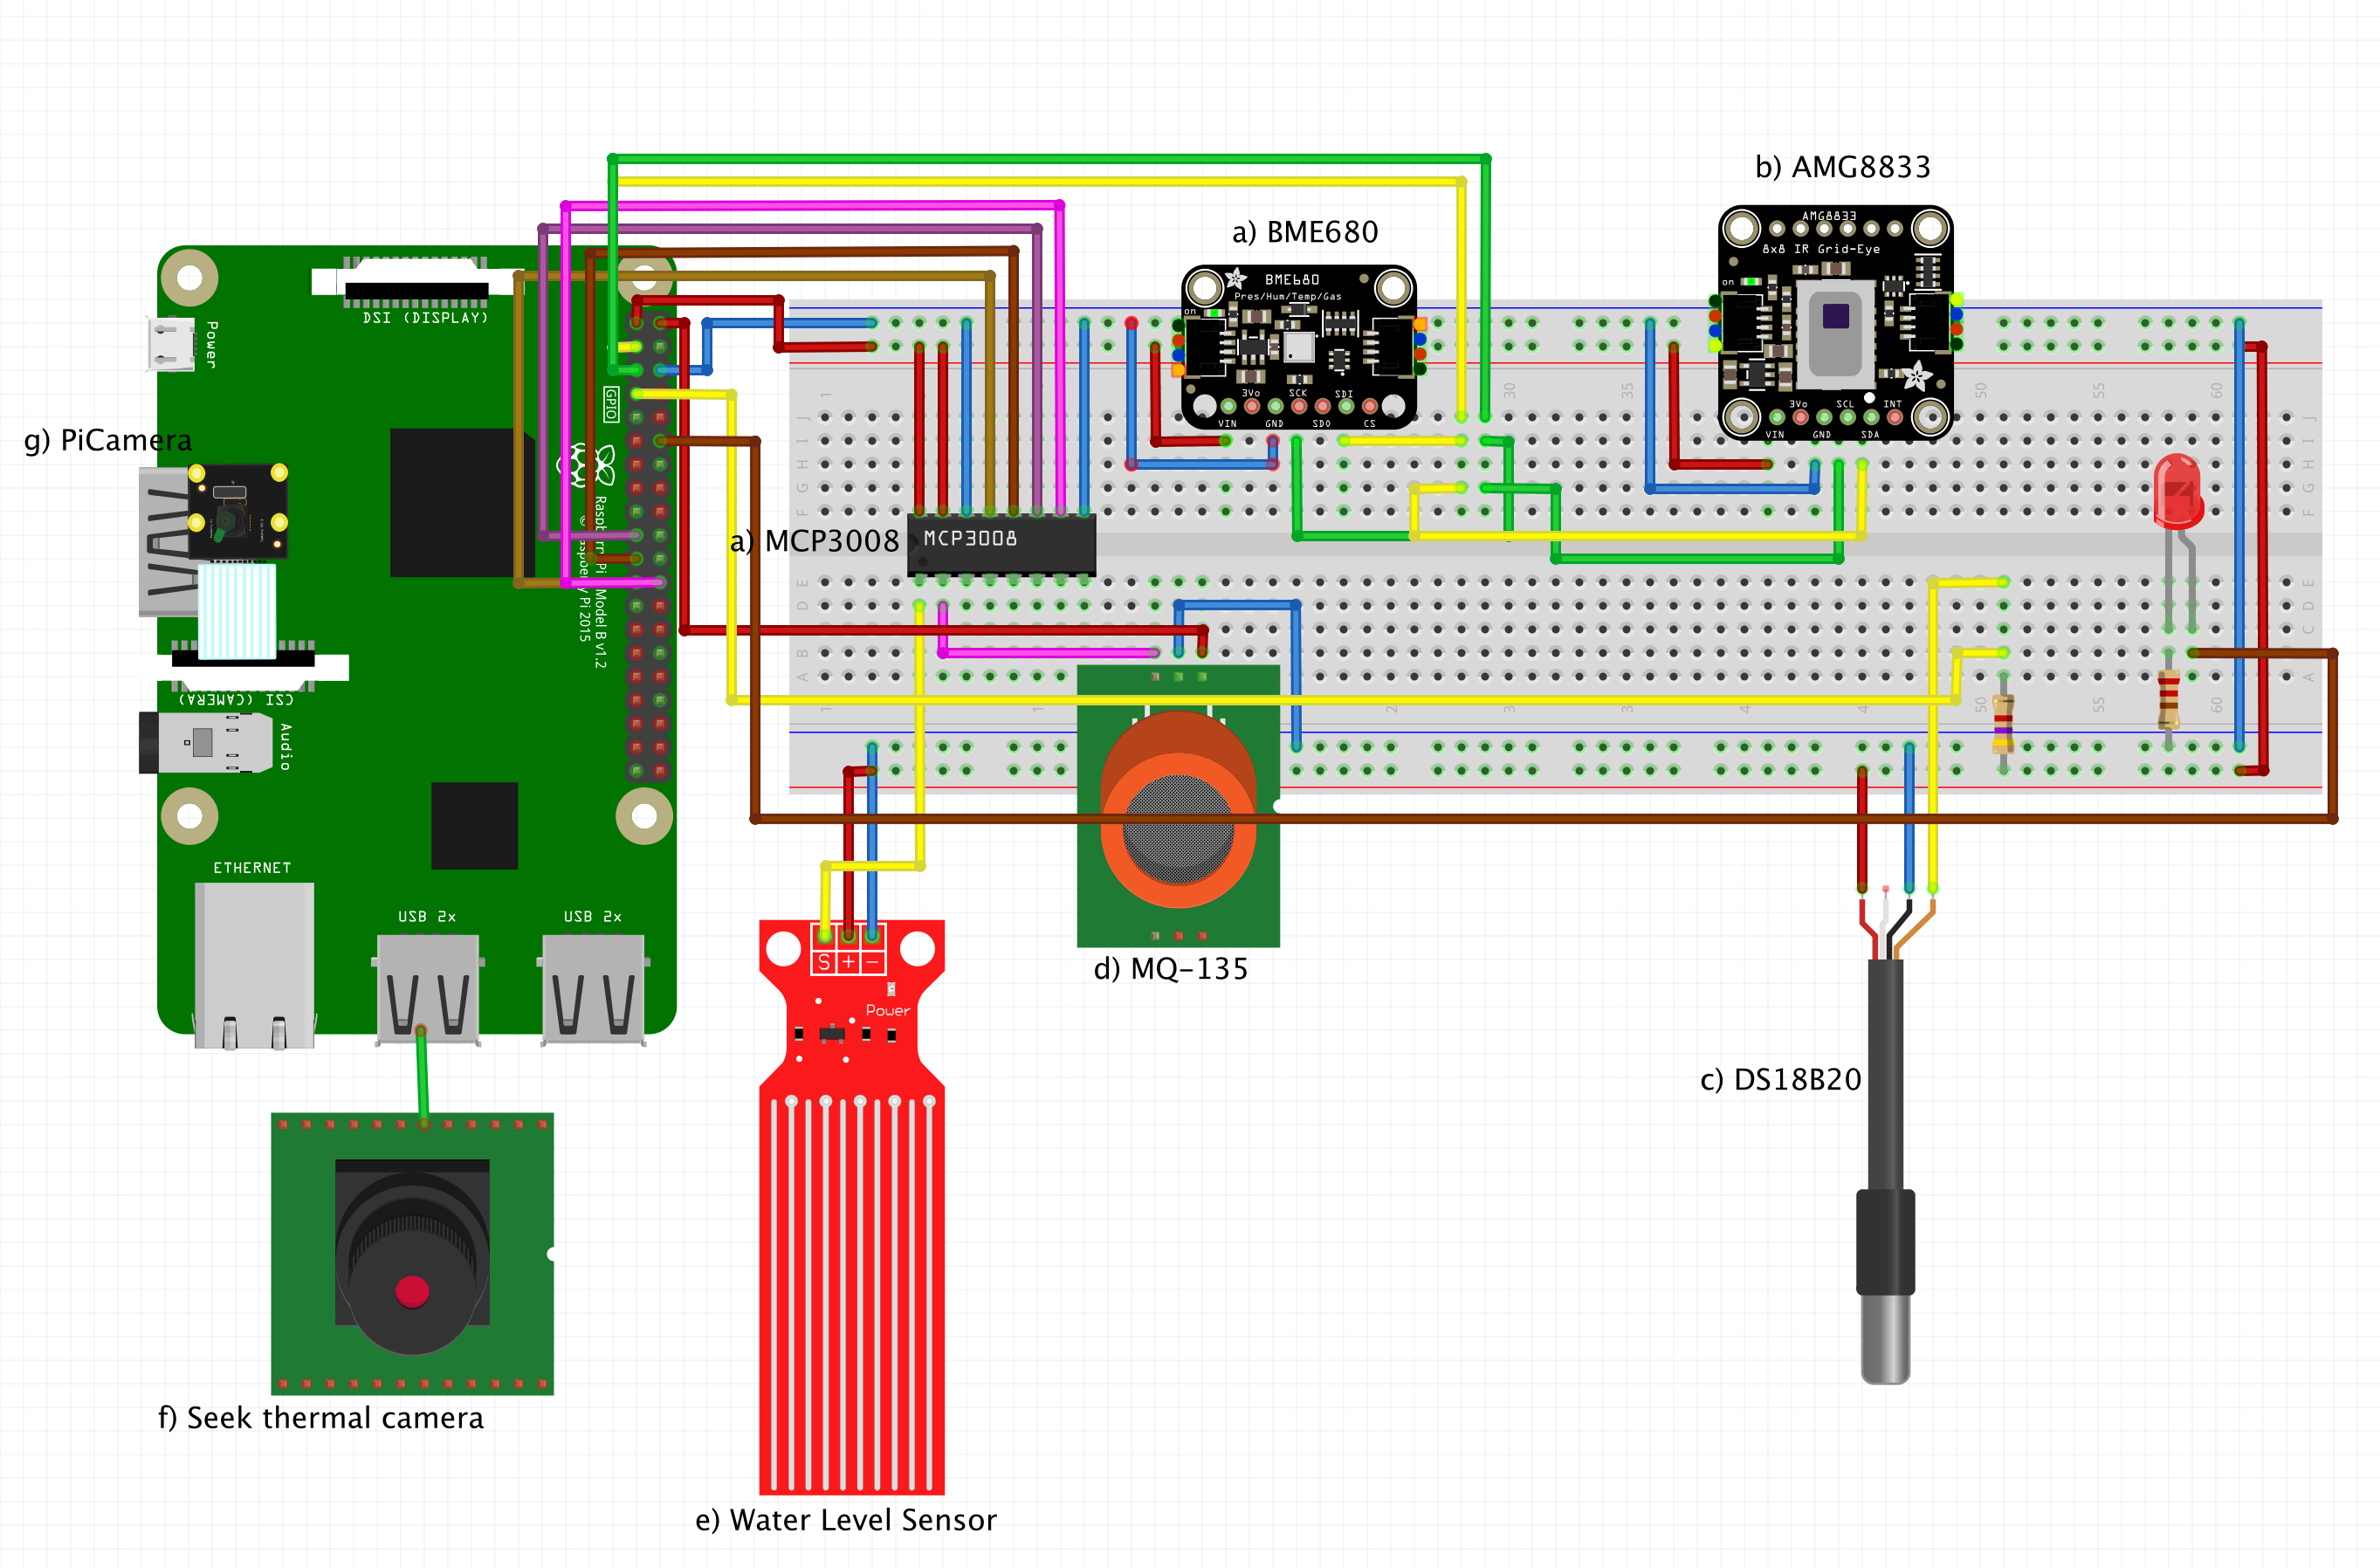
\includegraphics[width=10cm]{figs/conexiones}
\end{figure}
\note[item]{Se han conectado los sensores a la placa. Los sensores BME680 y AMG8833 requieren conexión con comunicación I2C, por lo que se han conectado a los pines pertinentes. Los sensores de nivel de agua y MQ-135 requieren de lecturas analógicas, por lo que se ha utilizado  un CAD. Las cámaras se ha conectado en los puertos pertinentes y el sensor de temperatura resistente al agua junto con una resistencia necesaria para medidas estables.}
\end{frame}

\subsection{Desarrollo software}
\begin{frame}
\frametitle{Desarrollo software}
\begin{enumerate}
\item Lectura sensorial con Python
\item Creación de la interfaz de usuario
\item Integración de las cámaras en la IU
\end{enumerate}
\begin{figure}
\centering
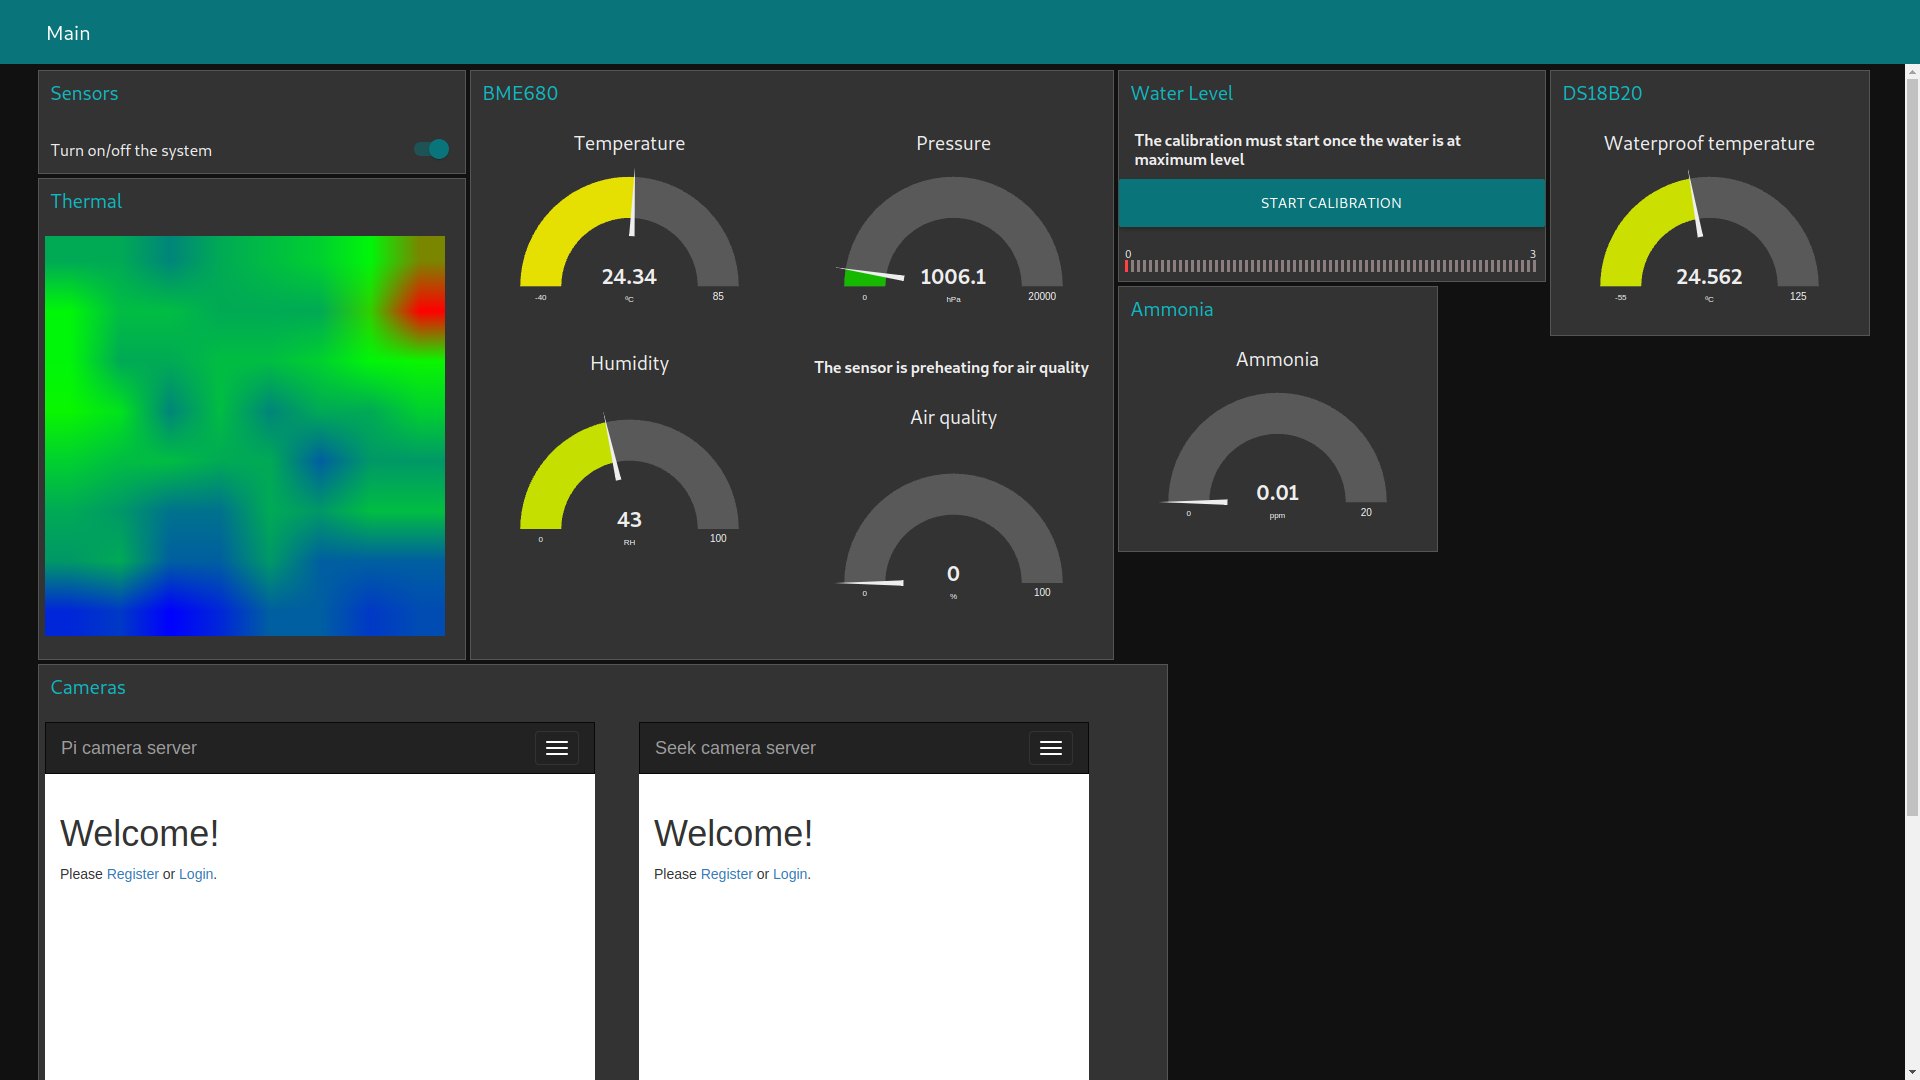
\includegraphics[width=10cm]{figs/UIcompleta}
\end{figure}
\note[item]{El primer paso, después de crear el diagrama de casos de uso así como el diagrama de clases del sistema, ha sido crear la lectura sensorial con Python. Con el uso de la librería Threads se ha conseguido leer de forma concurrente de todos los valores a la vez. Se han realizado algunos cambios en la lectura de los sensores, como en el caso del BME680 para que en lugar de mostrar la resistencia del aire se muestre la calidad de este en proporción a la humedad y resistencia del aire.\\

Una vez se ha obtenido este fichero, se ha procedido a la creación de la interfaz de usuario en Node-Red. Para ello, ha sido necesario combinar distintos tipos de nodos para la transformación de valores numéricos a la representación de ellos en widgets. En algunos casos, como en el del sensor AMG8833 (el sensor térmico) se han requerido más nodos para convertir el mapa en una imagen con una resolución mejor.\\

Con el uso de Flask, se han creado dos servidores: uno para cada cámara. De esta manera, se han podido incorporar a la interfaz de Flask a través del nodo template, que permite mostrar una url. Con Flask también se ha incorporado un botón que permite iniciar o parar la grabación de la PiCam. Además, se han añadido algunas mejoras con el uso de OpenCV a la visualización de las cámaras, como el timestamp.}
\end{frame}

\begin{frame}
\frametitle{Seguridad}
\begin{itemize}
\item Servidores con login y 2FA
\item Login en el flujo de Node-Red así como en la interfaz de usuario
\item Cambio de HTTP a HTTPS
\end{itemize}
\note[item]{Debido a la existencia de servidores, así como el acceso al flujo de nodos de Node-Red y la interfaz de usuario, ha sido necesario dotar al sistema de más seguridad. En primer lugar, a los servidores se han añadido un login necesario basado en el factor de doble autenticación; con usuario, contraseña y un código de 30 segundos de vida.\\

De la misma forma se ha añadido un login necesario al flujo de nodos así como a la interfaz de usuario. Es importante marcar que dichos login son diferentes, pues al primero solo podrá acceder el administrador, quien debe tener conocimiento para modificar cualquier nodo, y al segundo, cualquier usuario autorizado.\\

Finalmente, tanto Node-Red como los servidores se encontraban bajo direcciones de HTTP. Esto se ha modificado a HTTPS bajo unos certificados autofirmados.}
\end{frame}

\begin{frame}
\frametitle{Autoarranque}
\begin{figure}
\centering
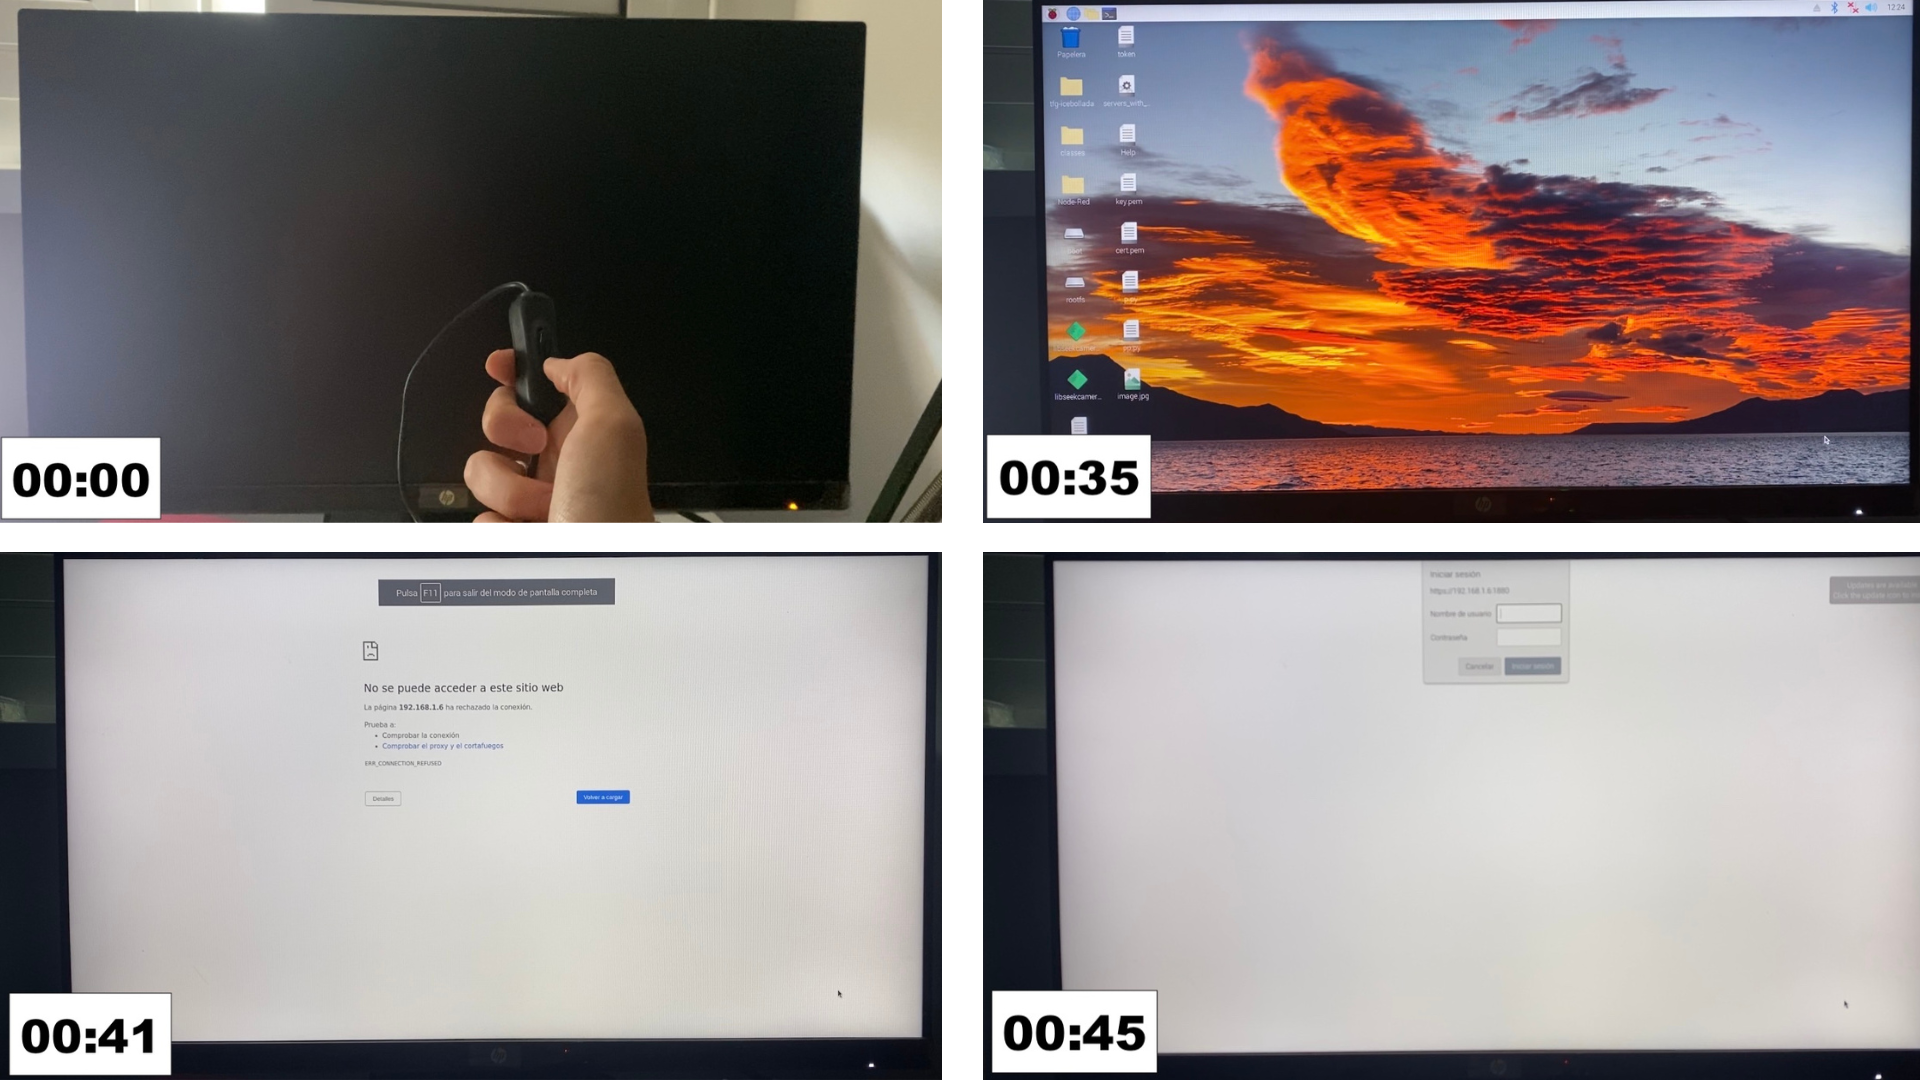
\includegraphics[width=12cm]{figs/autoarranque}
\end{figure}
\note[item]{Por último, se ha adaptado el sistema de acuerdo a uso de un usuario ajeno a cualquier conocimiento de robótica. De esta manera, cuando se enciende la placa Raspberry el sistema se lanza automáticamente, de forma que la pantalla que recibe el usuario es la solicitud de datos para acceder a la interfaz.}
\end{frame}

\begin{frame}
\frametitle{Detección de ratones mediante técnicas de Deep Learning}
\begin{figure}
\centering
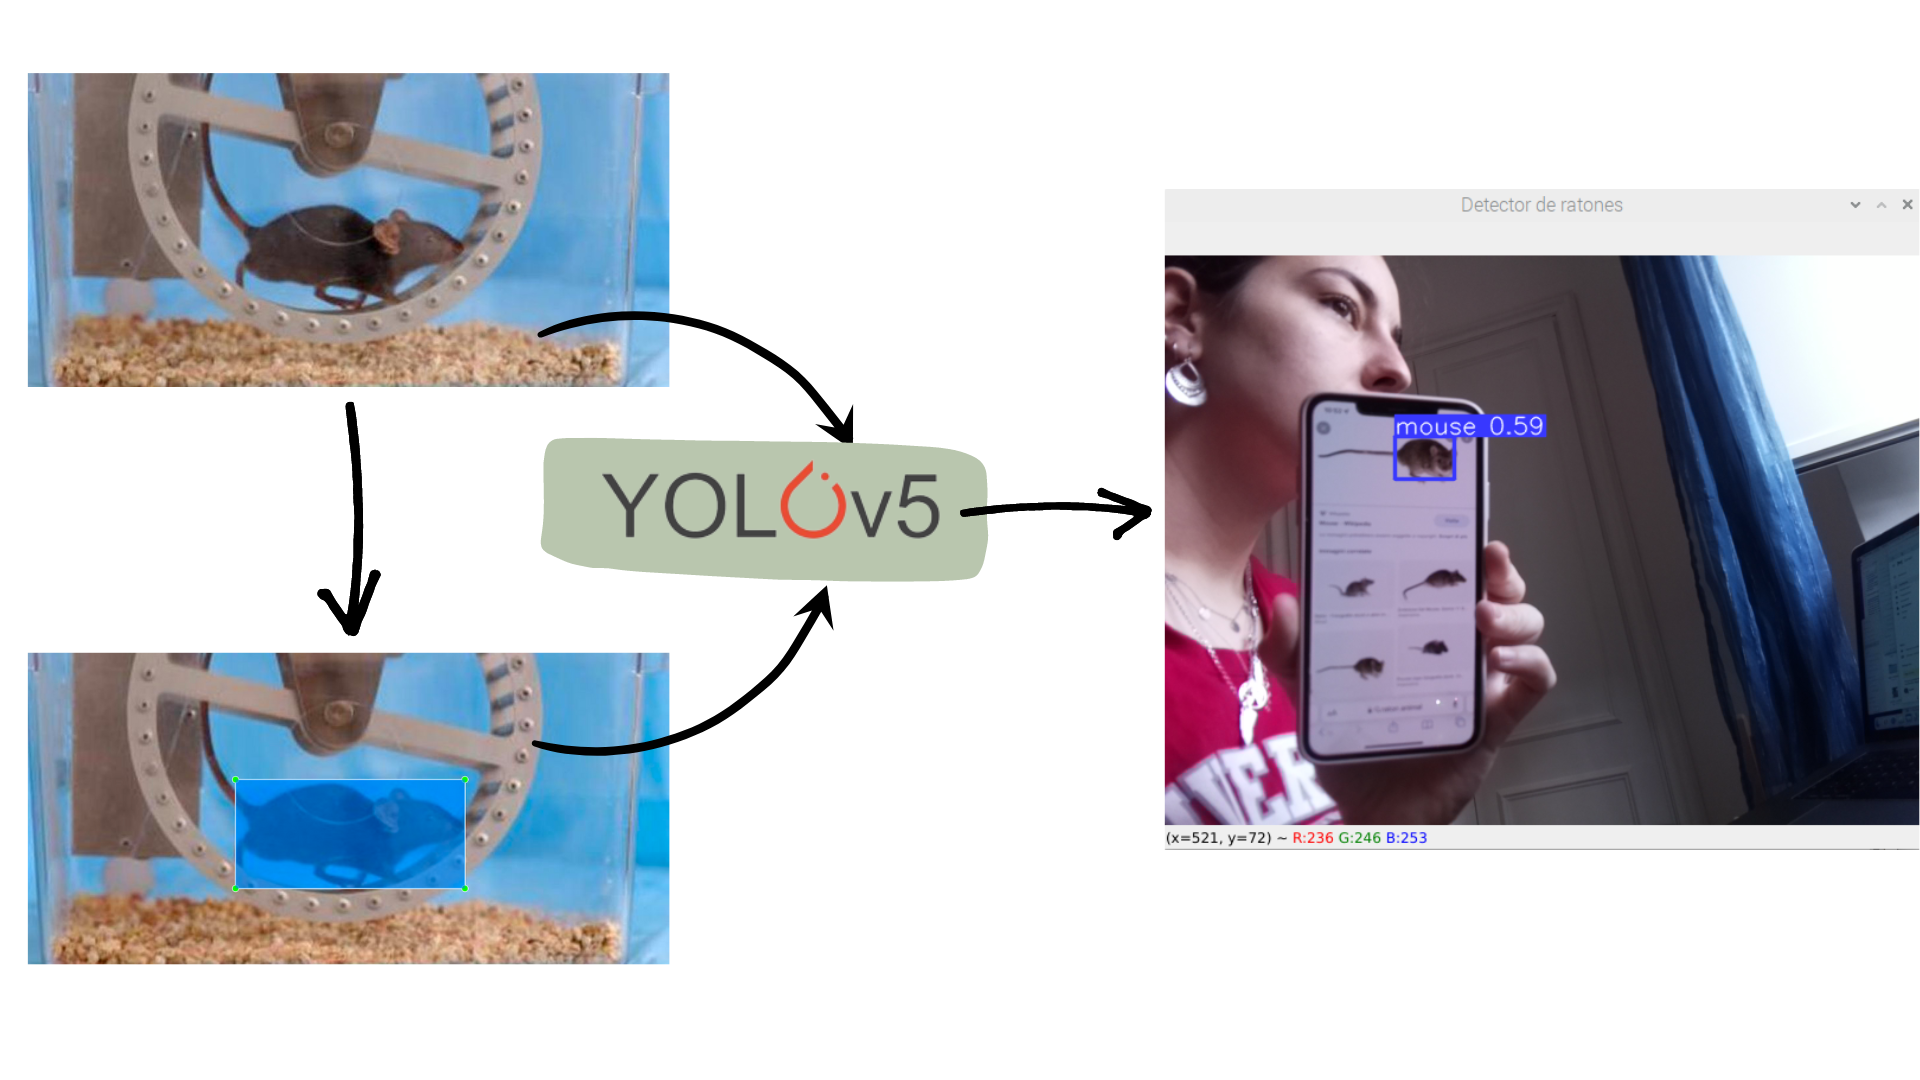
\includegraphics[width=12cm]{figs/deteccion-2}
\end{figure}
\note[item]{Cumpliendo el tercer objetivo comentado, se ha creado un modelo para la detección de ratones. Para ello, ha sido necesario crear un dataset, dado que no se ha encontrado ninguno cercano a los objetivos en Internet. El dataset creado consta de 354 imágenes: 275 para el proceso de entrenamiento y 79 para el de validación. Una vez se ha obtenido el dataset, se han etiquetado todas las imágenes en formato YOLO.\\

Después se ha entrenado el modelo con el dataset y las etiquetas creadas. Para elegir el mejor modelo, se han probado distintos modelos de YOLO, desde el más rápido y menos preciso hasta el más lento y más preciso. Después de observar el comportamiento de los distintos modelos creados tanto en raspberry como en un ordenador normal, se ha decidido optar por el modelo YOLOv5s, uno de los más rápidos (pero también menos preciso) dado que el rendimiento de la CPU de rapsberry es más limitado que un ordenador normal. Aun así, el flujo de las imágenes no es en tiempo real, y la detección no es del todo precisa.}
\end{frame}

%-----------------------------------------------------------------------CONCLUSIONES---------------------------------------------------------------------------------------
\section*{}
\begin{frame}{}
  \centering \Huge
  \emph{Conclusiones}
\note[item]{Para acabar esta presentación, vamos a repasar lo hecho, unas breves conclusiones y las líneas futuras.}
\end{frame}

\section{Conclusiones}
\begin{frame}
\frametitle{Conclusiones}
\begin{block}{Objetivos cumplidos}
\begin{itemize}
\item Interfaz de usuario creado en Node-Red .
\item Detección de ratones mediante algoritmo de Deep Learning.
\item El sistema funciona en tiempo real en Raspberry: sistema \textit{low-cost}.
\item Interfaz para el usuario final.
\item Accesible desde cualquier dispositivo de la misma red.
\end{itemize}
\note[item]{La interfaz de usuario se ha creado en Node-Red a partir del fichero de lectura de sensores concurrentes y los servidores de las cámaras. También se ha conseguido la detección de ratones en la raspberry, a pesar de que no es en tiempo real.\\

Además, se ha conseguido que sea un sistema low-cost al trabajar con Raspberry y sensores baratos. La interfaz es una interfaz intuitiva para cualquier perfil de usuario, y es accesible desde cualquier dispositivo conectado a la misma red que la raspberry.}
\end{block}

\begin{block}{Líneas futuras}
\begin{itemize}
\item Adaptación de la IU a un servidor accesible desde cualquier lugar.
\item Análisis del comportamiento de los animales con técnicas de DL.
\item Creación de un Docker para la instalación por cualquier usuario.
\end{itemize}
\note[item]{Finalmente, algunas de las líneas futuras para finalizar este trabajo son:\\

Adaptar la IU a un servidor accesible desde cualquier lugar y no solo desde la misma red que raspberry.\\

Analizar el comportamiento de los ratones con el modelo de detección de ratones creado, para analizar cuánto tiempo pasan realizando las diferentes actividades así como en las distintas cubetas.\\

Y la creación de un Docker para permitir la instalación a cualquier usuario que no tiene por qué tener conocimiento sobre el tema.}
\end{block}
\end{frame}

\begin{frame}[plain]
\large{\titlepage}
\note[item]{Y hasta aquí mi exposición.}
\note[item]{Quedo a disposición del tribunal para cualquier duda que tenga.}
\end{frame}
\endgroup
\end{document}
